\documentclass[frontgrid]{flacards}
\usepackage{color}

% For circuit diagrams
\usepackage{circuitikz}

% For awkward circuit diagrams
\usepackage{tikz}
\usetikzlibrary{shapes}
\usetikzlibrary{arrows}
\usetikzlibrary{circuits}

\definecolor{light-gray}{gray}{0.75}

\newcommand{\frontcard}[1]{\textcolor{light-gray}{\colorbox{light-gray}{$#1$}}}
\newcommand{\backcard}[1]{#1} 

\newcommand{\flashcard}[1]{% create new command for cards with blanks
    \card{% call the original \card command with twice the same argument (#1)
        \let\blank\frontcard% but let \blank behave like \frontcard the first time
        #1
    }{%
        \let\blank\backcard% and like \backcard the second time
        #1
    }%
}

\begin{document}

\pagesetup{2}{4} 

\card{
	What is a hierarchy?
}{
	A hierarchy is a group of objects arranged in tiers of descending magnitude,
	importance or complexity.
}

\card{
	Define {\it digital}.
}{
	An entity that can reside in one of two states at any one time.
}

\card{
	Define {\it analogue}.
}{
	An entity that can reside in an infinite number of possible states.
}

\card{
	How many values can be represented by a binary number containing $n$ bits?
}{
	$2^n$
}

\card{
	Arrange {\tt AND}, {\tt OR} and {\tt NOT} in order of operator precedence.
}{
	{\tt NOT}, {\tt AND}, {\tt OR}
}

\card{
	What is the symbol for {\tt AND}? 
}{
	$\cdot$
	\\
	E.g. $A \cdot B$
}

\card{
	What is the symbol for {\tt OR}?
}{
	$+$
	\\
	E.g. $A + B$
}

\card{
	What is the symbol for {\tt NOT}
}{
	$\overline{\phantom{A}}$
	\\
	E.g. $\overline{A}$
}

\card{
	What is the symbol for {\tt XOR}
}{
	$\oplus$
	\\
	E.g. $A \oplus B$
}

\card{
	What is De Morgan's theorem commonly used for when designing digital 
	circuits?
}{
	Converting gates such as {\tt AND}, {\tt OR}, {\tt XOR} etc into {\tt NAND}
	and {\tt NOR} since they are cheap and fast.
}

\card{
	What is the symbol for an {\tt AND} gate?	
}{
	\begin{circuitikz} \draw
		(0,0) node[and port] (and) {};
	\end{circuitikz}
}

\card{
	What is the symbol for an {\tt OR} gate?	
}{
	\begin{circuitikz} \draw
		(0,0) node[or port] (or) {};
	\end{circuitikz}
}

\card{
	What is the symbol for an {\tt XOR} gate?	
}{
	\begin{circuitikz} \draw
		(0,0) node[xor port] (xor) {};
	\end{circuitikz}
}

\card{
	What is the symbol for an {\tt NOT} gate?	
}{
	\begin{circuitikz} \draw
		(0,0) node[not port] (not) {};
	\end{circuitikz}
}

\card{
	What is the symbol for an {\tt NAND} gate?	
}{
	\begin{circuitikz} \draw
		(0,0) node[nand port] (nand) {};
	\end{circuitikz}
}

\card{
	What is the symbol for an {\tt NOR} gate?	
}{
	\begin{circuitikz} \draw
		(0,0) node[nor port] (nor) {};
	\end{circuitikz}
}

\card{
	What's the symbol for a n:1 multiplexer?
}{
	% I can't find a way to draw it in LaTeX...
	\centering\fbox{
		\begin{minipage}{2in}
			\hfill\vspace{1in}
		\end{minipage}
	}
}

\flashcard{
	What is the truth table for binary addition?
	\begin{tabular}{|c c c|c c|}
		\hline
		$A$ & $B$ & $c_{in}$ & $S$ & $c_{out}$\\ \hline
		0 & 0 & 0 & \blank{0} & \blank{0}\\
		0 & 0 & 1 & \blank{1} & \blank{0}\\
		0 & 1 & 0 & \blank{1} & \blank{0}\\
		0 & 1 & 1 & \blank{0} & \blank{1}\\
		1 & 0 & 0 & \blank{1} & \blank{0}\\
		1 & 0 & 1 & \blank{0} & \blank{1}\\
		1 & 1 & 0 & \blank{0} & \blank{1}\\
		1 & 1 & 1 & \blank{1} & \blank{1}\\ \hline
	\end{tabular}
}

\card{
	How do you negate a binary number?
}{
	1. Invert the bits\\
	2. Add 1
}

\card{
	Convert binary $6$ to $-6$
}{
	1. Start with {\tt 0110}\\
	2. Invert the bits - {\tt 1001}\\
	3. Add 1 - {\tt 1010}
}


\card{
	Which bit is the signed bit when using 2's complement?
}{
	The left most bit.
}

\card{
	How do you subtract two binary numbers?
}{
	1. Invert the number you're subtracting\\
	2. Add 1 to the inverted number\\
	3. Add the number you're subtracting from with the inverted number.\\
	Basically, add the original number to the 2's complement negative of what
	you're taking away.
}

\card{
	What is the {\it sum-of-products}?
}{
	When a number of {\tt AND} gates are {\tt OR}'ed together.
}

\card{
	What is the {\it product-of-sums}?
}{
	When a number of {\tt OR} gates are {\tt AND}'ed together.
}

\card{
	What is the structure of a half adder (in terms of gates)?
}{
	\begin{circuitikz} \draw
	(0,2) node[and port] (and1) {}
	(0,0) node[and port] (and2) {}
	(2,1) node[or port] (or) {}
	(1, -2) node[and port] (and3) {}
	(and1.in 1) node[anchor=east] {$\overline{A}$}
	(and1.in 2) node[anchor=east] {B}
	(and2.in 1) node[anchor=east] {A}
	(and2.in 2) node[anchor=east] {$\overline{B}$}
	(and1.out) -- (or.in 1)
	(and2.out) -- (or.in 2)
	(or.out) node[anchor=west] {S}
	(and3.in 1) node[anchor=east] {A}
	(and3.in 2) node[anchor=east] {B}
	(and3.out) node[anchor=west] {$c_{out}$};
	\end{circuitikz}
}

\flashcard{
	What is the truth table for the half adder?
	\begin{tabular}{|c c |c c|}
		\hline
		$A$ & $B$ & $S$ & $c_{out}$\\ \hline
		0 & 0 & \blank{0} & \blank{0}\\
		0 & 1 & \blank{1} & \blank{0}\\
		1 & 0 & \blank{1} & \blank{0}\\
		1 & 1 & \blank{0} & \blank{1}\\ \hline
	\end{tabular}	
}

\card{
	Define propagation delay.
}{
	Propagation delay is the time taken for the output of a gate to change after
	it's inputs have changed.
}

\flashcard{
	Fill in the table:
	\begin{tabular}{|c|c|}
		\hline
		State & Symbol \\ \hline
		Low      & \blank{0}\\
		High     & \blank{1}\\
		Tristate & \blank{Z}\\
		Unknown  & \blank{X}\\ \hline
	\end{tabular}	
}

\card{
	What does active high and active low mean?
}{
	If a signal is active high, then it is interpreted as {\tt True} when the
	signal is high (e.g. a light is on, or the voltage is positive etc).\\
	If a signal is active low, then it is interpreted as {\tt True} when the
	signal is low (e.g. a light is off, or the voltage is negative etc).
}

\card{
	What are the advantages of a hierarchy:
}{
	1. Encapsulation\\
	2. Reuse of logic\\
	3. Only have to define and test things once
}

\card{
	What is a combinatorial circuit?
}{
	A circuit where the value of the output depends only on the values of the
	input.
}

\card{
	What is a sequential circuit?
}{
	A circuit where the value of the output depends on the values of the input
	and the past history of it's inputs. A sequential circuit requires a clock
	and memory.
}

\card{
	What is a synchronous clock?
}{
	A synchronous clock is one that is effective system wide; all components in
	the system adhere to this clock.
}

\card{
	What is a clock edge?
}{
	The point on a clock signal where the signal is going from low to high 
	(rising or positive edge) or high to low (falling or negative edge.)
}

\card{
	Define bistable.
}{
	An entity that can be in one of two stable states.
}

\card{
	What is a flip flop?
}{
	A bistable device that latches onto a state.
}

\card{
	What is a register made of?
}{
	A series of flip flops, each containing one bit.
}

\card{
	What is a finite state machine?
}{
	A digital system that holds the current state of itself and progresses to a
	new state based on the value of the current state.
}

\card{
	What do {\tt S} and {\tt R} stand for on a S-R flip flop?
}{
	{\tt S} - Set\\
	{\tt R} - Reset
}

\card{
	What is the circuit symbol for a D-type latch?
}{
	\begin{tikzpicture}
		\draw (0,0) rectangle (2,2);
		\draw (0,1.5) -- (-1,1.5);
		\draw (2,0.5) -- (3,0.5);
		\draw (2,1.5) -- (3,1.5);
		\draw (1,0) -- (1,-1);
		\filldraw[fill=white] (2.04, 0.5) circle (1pt);
		\node at (0.2, 1.5) {D};
		\node at (1, 0.2) {En};
		\node at (1.8, 1.5) {Q};
		\node at (1.8, 0.5) {$\overline{Q}$};
	\end{tikzpicture}
}

\card{
	What is the structure of a D-type flip flop?
}{
	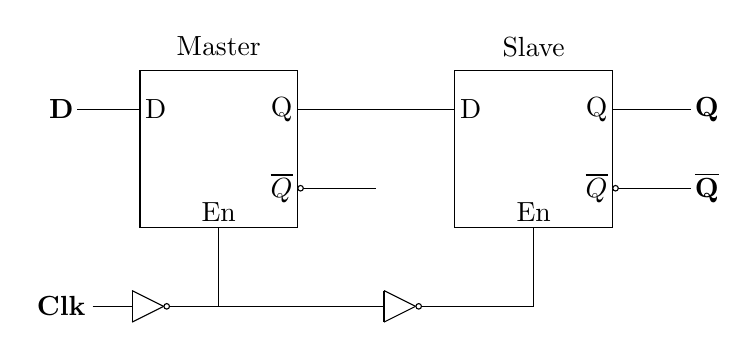
\begin{tikzpicture}
		\draw (0,0) rectangle (2,2);
		\draw (0,1.5) -- (-0.8,1.5);
		\draw (2,0.5) -- (3,0.5);
		\draw (2,1.5) -- (3,1.5);
		\draw (1,0) -- (1,-1);
		\filldraw[fill=white] (2.04, 0.5) circle (1pt);
		\node at (0.2, 1.5) {D};
		\node at (1, 0.2) {En};
		\node at (1.8, 1.5) {Q};
		\node at (1.8, 0.5) {$\overline{Q}$};

		\draw (4,0) rectangle (6,2);
		\draw (4,1.5) -- (3,1.5);
		\draw (6,0.5) -- (7,0.5);
		\draw (6,1.5) -- (7,1.5);
		\draw (5,0) -- (5,-1);
		\filldraw[fill=white] (6.04, 0.5) circle (1pt);
		\node at (4.2, 1.5) {D};
		\node at (5, 0.2) {En};
		\node at (5.8, 1.5) {Q};
		\node at (5.8, 0.5) {$\overline{Q}$};


		% Not gate
		\draw (-0.1,-0.8) -- (-0.1,-1.2);
		\draw (-0.1,-0.8) -- (0.3,-1);
		\draw (-0.1,-1.2) -- (0.3,-1);
		\filldraw[fill=white] (0.34, -1) circle (1pt);
		% Not gate 2
		\draw (3.1,-0.8) -- (3.1,-1.2);
		\draw (3.1,-0.8) -- (3.5,-1);
		\draw (3.1,-1.2) -- (3.5,-1);
		\filldraw[fill=white] (3.54, -1) circle (1pt);
		\draw (-0.6, -1) -- (-0.1, -1);
		\draw (0.38, -1) -- (3.1, -1);
		\draw (3.58, -1) -- (5, -1);

		\node at (-1, -1) {{\bf Clk}};
		\node at (-1, 1.5) {{\bf D}};
		\node at (7.2, 1.5) {{\bf Q}};
		\node at (7.2, 0.5) {{$\overline{\textrm{\bf Q}}$}};

		\node at (1, 2.3) {Master};
		\node at (5, 2.3) {Slave};
	\end{tikzpicture}
}

\card{
	Is a D-type latch level sensitive or edge sensitive? What does that mean?
}{
	The D-type latch is level sensitive, meaning that it will change state 
	whenever the input changes, this means it's {\bf asynchronous}.
}

\card{
	What is the circuit symbol for a D-type flip flop?
}{
	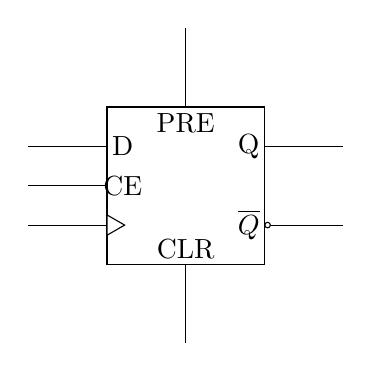
\begin{tikzpicture}
		\draw (0,0) rectangle (2,2);
		\draw (0,1.5) -- (-1,1.5);
		\draw (0,1) -- (-1,1);
		\draw (0,0.5) -- (-1,0.5);
		\draw (2,0.5) -- (3,0.5);
		\draw (2,1.5) -- (3,1.5);
		\draw (1,0) -- (1,-1);
		\draw (1,2) -- (1,3);
		\filldraw[fill=white] (2.04, 0.5) circle (1pt);
		\node at (0.2, 1.5) {D};
		\node at (1, 0.2) {CLR};
		\node at (1, 1.8) {PRE};
		\node at (0.2, 1) {CE};
		\node[fill=white, draw=black, rotate=-90,regular polygon, regular 
			  polygon sides=3,inner sep=1.5pt] at (0.075, 0.5) {};
		\node at (1.8, 1.5) {Q};
		\node at (1.8, 0.5) {$\overline{Q}$};
	\end{tikzpicture}
}

\card{
	What does a D-type flip flop implement to make it synchronous?
}{
	It has an enable switch that can be linked to the clock so that it will
	only change state when the device is clocked.
}

\card{
	What are the three delays in the D-type flip flop?
}{
	The set-up time ($T_{SU}$), the hold time ($T_{H}$) and the
	propagation delay ($T_{PD}$).
}

\card{
	In order to ensure that a D-type flip flop will change state successfully, 
	when does the input have to be constant?
}{
	From the beginning of the set-up time to the end of the hold time.
}

\card{
	What is the propagation delay?
}{
	The time taken for the flip flop to output a change of state.
}

\card{
	What is edge speed?
}{
	The time taken for a signal to change state.
}

% Second book of Paul's notes (pink)

\card{
	What does RTL mean?
}{
	Register Transfer Layer
}

\card{
	Order the following in terms of their level of abstraction from lowest to
	highest:\\
	$\cdot$ Logic Gate Level\\
	$\cdot$ Transistor Level\\
	$\cdot$ Register Transfer Level
}{
	$1$ Transistor Level\\
	$2$ Logic Gate Level\\
	$3$ Register Transfer Level
}

\card{
	What does the CE pin do on a register?
}{
	CE stands for clock enable, and when it is low, the register will ignore 
	clock cycles.
}

\card{
	What are registers made up of?
}{
	Lots of flip flops.
}

\card{
	Define the datapath.
}{
	The datapath is the path of registers and logical functions that the data 
	flows through.
}

\card{
	What does the control block do at the Register Transfer Level?
}{
	The control block controls the operation of the datapath. It sends control 
	signals to the datapath so that the data does indeed, take the right path.
}

\card{
	What data flows between the datapath and the control block?
}{
	The control block gives the datapath control inputs.\\
	The datapath gives control outputs to the control block.
}

\card{
	For a finite state machine with $n$ states, how many flip flops are needed 
	in the register?
}{
	At least $\log_2{n}$
}

\card{
	What is this an example of:\\
	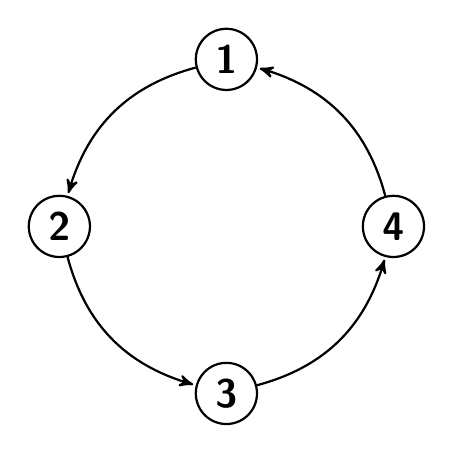
\begin{tikzpicture}[->,>=stealth',shorten >=1pt,auto,node distance=3cm,
                    thick,main node/.style={circle,draw,font=\sffamily\Large\bfseries}]

		\node[main node] (1) {1};
		\node[main node] (2) [below left of=1] {2};
		\node[main node] (3) [below right of=2] {3};
		\node[main node] (4) [below right of=1] {4};

		\path[every node/.style={font=\sffamily\small}]
		(1) edge [bend right] node[left] {} (2)
		(2) edge [bend right] node[left] {} (3)
		(3) edge [bend right] node[right] {} (4)
		(4) edge [bend right] node[right] {} (1);
	\end{tikzpicture}
}{
	A state transition diagram.
}

\card{
	What is the synchronous paradigm?
}{
	When all state changes in a system happen at once (usually at the same time
	as a clock transition).
}

\card{
	What is the formula to subtract $A$ from $B$ using 2's complement?
}{
	$A - B = A + \overline{B} + 1$
}

\end{document} 